\documentclass[12pt,journal]{IEEEtran}
\usepackage[letterpaper, margin=0.8in]{geometry}
\usepackage{framed, listings, graphicx}

\begin{document}

\title{reWRITE}

\author{EE149/249A Project Report, Fall 2015

Reia Cho, Christian (CJ) Geering, Nathaniel Mailoa, Rachel Zhang}


% make the title area
\maketitle

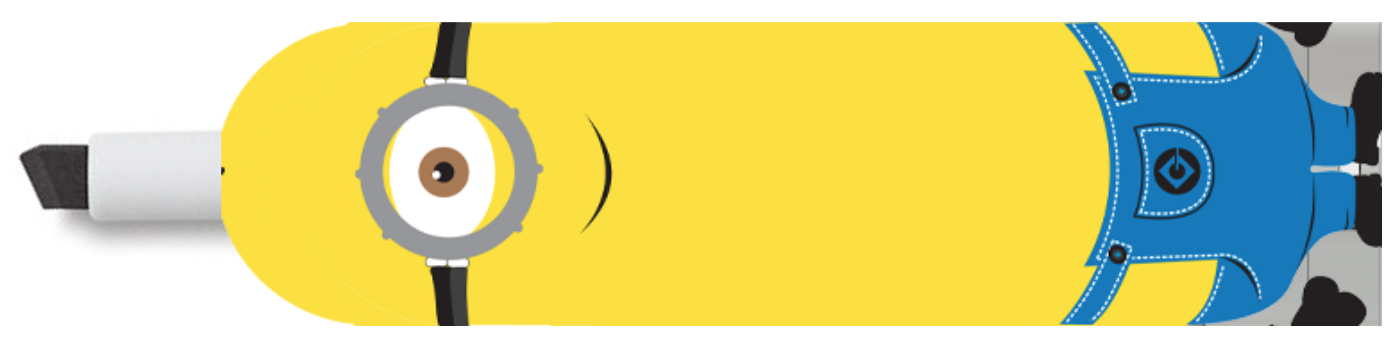
\includegraphics[width=\linewidth]{figures/minion}

\section{Introduction}


\section{Bill of Materials}


\section{System}
\subsection{LightBlue Bean}
\subsection{BNO055 Absolute Orientation Sensor Breakout Board}
\subsection{Li-Ion Battery}
\subsection{Force Sensor}
\subsection{Button and LED Sequin}

\section{Casing}

\section{Position Reconstruction}
\subsection{IMU Sensor Data}
\subsection{Filtering and Thresholding}
\subsection{Transformation to Fixed Reference Frame}
\subsection{Velocity Adjustment}
\subsection{Tip Position Reconstruction}
\subsection{Plotting}

\section{Quantitative Analysis and Scheduling}

\section{Mode of Operation}

\section{Acknowledgements}
We would like to acknowledge the following individuals for their support and contribution in this project.
\begin{itemize}
\item Trung Tran, \textit{National Instruments}
\item Prof. Sanjit Seshia, \textit{UC Berkeley}
\item Matthew Weber, \textit{UC Berkeley}
\item Eric Kim, \textit{UC Berkeley}
\item Casey Rogers, \textit{UC Berkeley 3D Modeling Club}
\end{itemize}

\newpage
\onecolumn

\section{Appendix 1: LightBlue Bean code}
\small{
\lstinputlisting[language=C,frame=single,breaklines=true]{stream_data.ino}
}

\section{Appendix 2: Python code}
\small{
\lstinputlisting[language=Python,frame=single,breaklines=true]{draw.py}
}

\end{document}



